\section{1174051 Evietania Charis Sujadi}
\subsection{Teori}
\subsubsection{Soal No. 1}
Kenapa file teks harus dilakukan tokenizer, dilengkapi dengan ilustrasi atau gambar.

Tokenizer adalah proses untuk membagi kalimat menjadi beberapa teks, hal ini sangat di perlukan dalam AI karena nanti setiap teks akan di hitung bobotnya dang akan memunculkan nilai vektor sehingga teks tersebut bisa di gunakan sebagai data untuk memprediksi teks yang muncul dalam satu kalimat sedangakan proses tkenizer merupakan caramembagi bagi teks dari suatu kalimat biasanya pembagi kalimat tersebut merupakan spasi dalan suatu kalimat.

\begin{itemize}
\item Ilustrasi Gambar:

\begin{figure}[H]
\centering
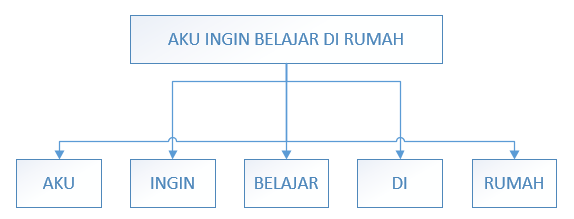
\includegraphics[scale=0.2]{figures/1174051/7/1.PNG}
\caption{Tokenizer}
\end{figure}

\end{itemize}

\subsubsection{Soal No. 2}
Konsep dasar K Fold Cross Validation pada dataset komentar Youtube, dilengkapi dengan ilustrasi atau gambar.
\begin{verbatim}
    kfold = StartifiedKFlod(n_splits=5)
    splits = kfold.split(d, d['CLASS'])
    \end{verbatim}
    pada codingan tersebut terdapat kfold sebagai variabel yang didalammnya terdiri dari split 5 yang berarti pengulangan terhadap pengolahan masing masing lima kali pada kasus ini terdapat data sebanyak 5 berarti ke lima data tersebut di ulang sebanyak lima kali dengan atribut class sebagai acuan pengolahan datanya kemudian akan di hasilkan akurasi dari pengulangan data tersebut sebesar sekian persen tergantung datanya.    
\begin{itemize}
\item Ilustrasi Gambar:
\begin{figure}[H]
\centering
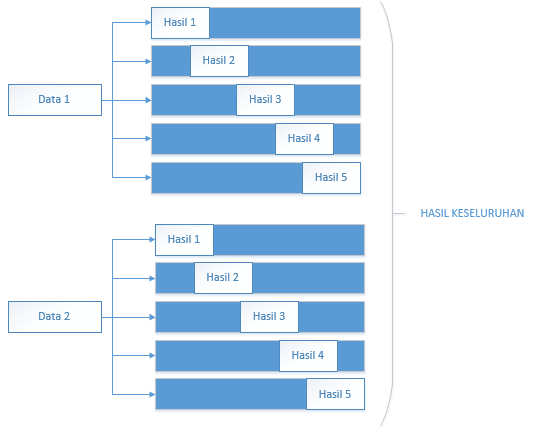
\includegraphics[scale=0.5]{figures/1174051/7/2.PNG}
\caption{Konsep dasar K Fold Cross Validation}
\end{figure}

\end{itemize}

\subsubsection{Soal No. 3}
Maksud kode program for train dan test in splits, dilengkapi dengan ilustrasi atau gambar.

Untuk melakukan pengujian atas data pada dataset sudah di tidak terjadi penumpukan dan split. Dimana di setiap class tidak akan muncul id yang sama.

\begin{itemize}
\item Ilustrasi Gambar :

\begin{figure}[H]
\centering
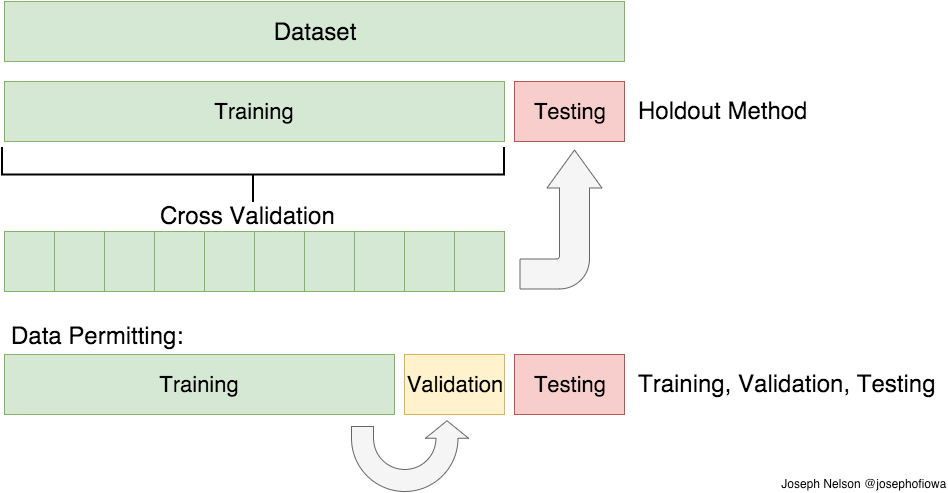
\includegraphics[scale=0.2]{figures/1174051/7/3.png}
\caption{Train dan Test in Split}
\end{figure}

\end{itemize}

\subsubsection{Soal No. 4}
Maksud kode program train content = d[’CONTENT’].iloc[train idx] dan test content = d[’CONTENT’].iloc[test idx], dilengkapi dengan ilustrasi atau gambar.

Untuk mengambil data pada kolom  CONTENT yang merupakan bagian dari train idx dan test idx.

\begin{itemize}
\item Ilustrasi Gambar:

\begin{figure}[H]
\centering
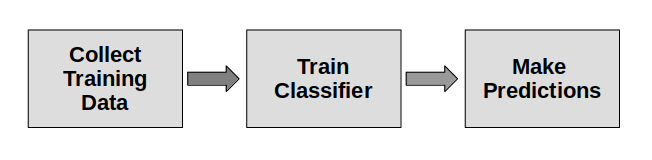
\includegraphics[scale=0.4]{figures/1174051/7/4.png}
\caption{Train content}
\end{figure}

\end{itemize}

\subsubsection{Soal No. 5}
Maksud dari fungsi tokenizer = Tokenizer(num words=2000) dan tokenizer.fit on texts(train content), dilengkapi dengan ilustrasi atau gambar.

Yang pertama, yaitu fungsi tokenizer ialah mem-vektorisasi jumlah kata yang ingin diubah kedalam bentuk token 2000 kata.

Yang kedua, untuk melakukan fit tokenizer untuk dat trainnya dengan data test nya untuk kolom CONTENT saja.

\begin{itemize}
\item Ilustrasi Gambar :

\begin{figure}[H]
\centering
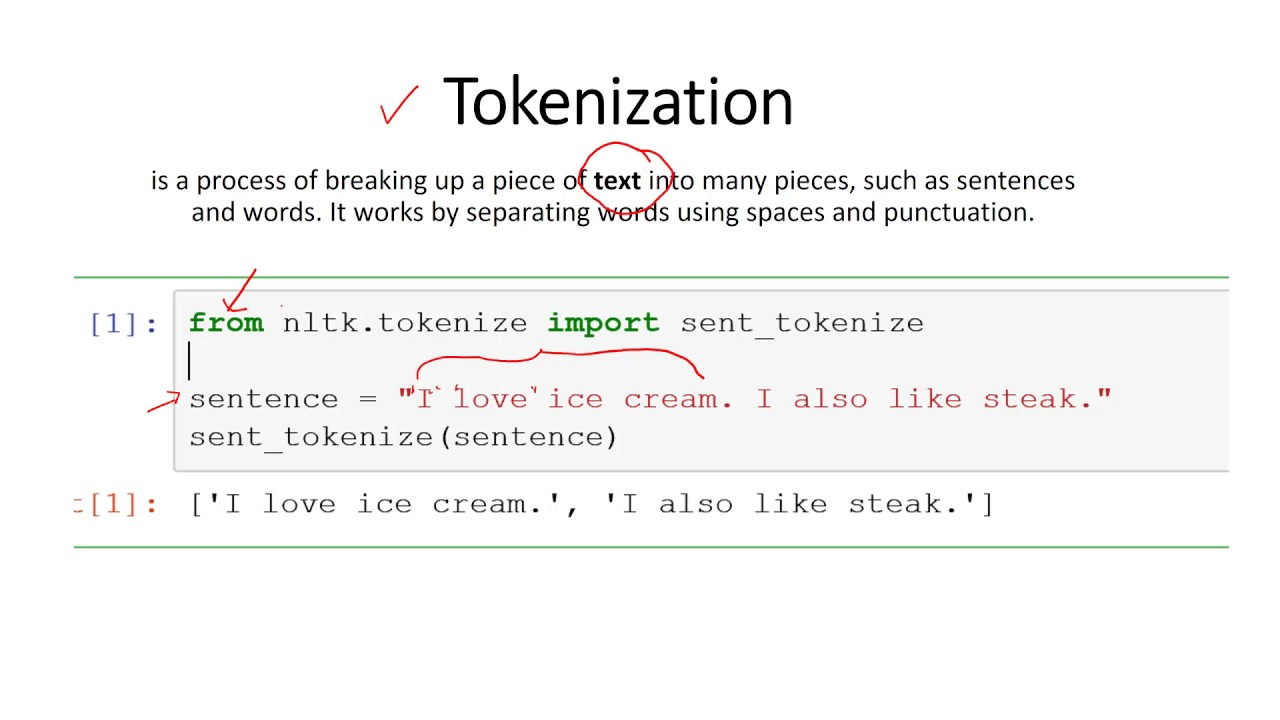
\includegraphics[scale=0.2]{figures/1174051/7/5.png}
\caption{Tokenizer}
\end{figure}

\end{itemize}

\subsubsection{Soal No. 6}
Maksud dari fungsi d train inputs = tokenizer.texts to matrix(train content, mode=’tfidf ’) dan d test inputs = tokenizer.texts to matrix(test content, mode=’tfidf ’), dilengkapi dengan ilustrasi atau gambar.

Variabel d train input untukmelakukan tokenizer dari bentuk teks ke matrix dari data train content dengan mode tfidf dan variabel d test inputs sama saja untuk data test.

\begin{itemize}
\item Ilustrasi Gambar:

\begin{figure}[H]
\centering
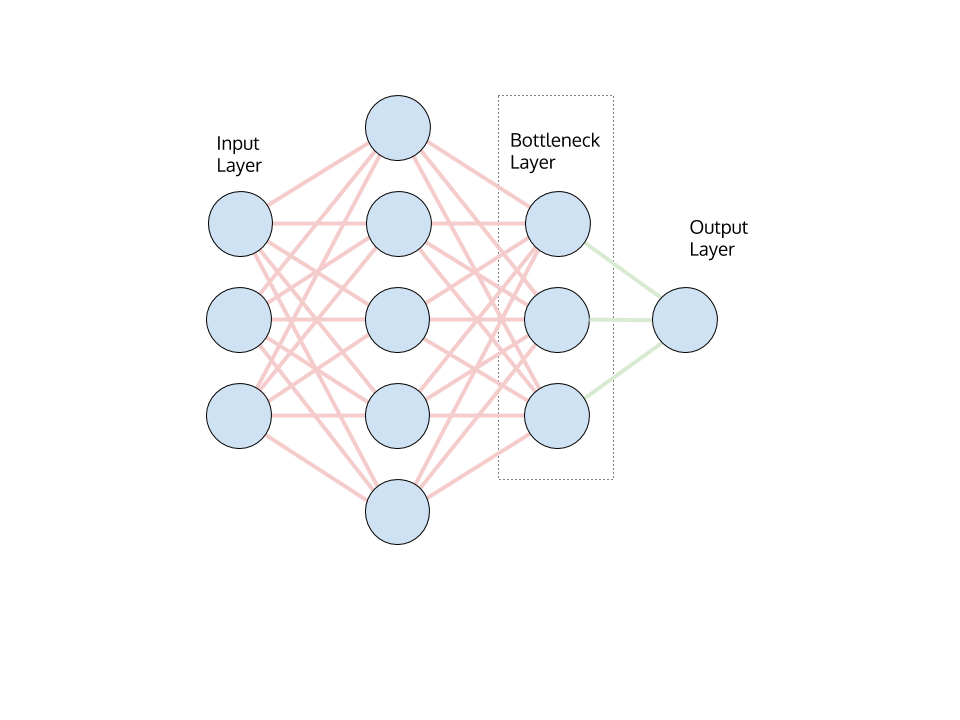
\includegraphics[scale=0.3]{figures/1174051/7/6.png}
\caption{Train Inputs 1}
\end{figure}

\end{itemize}

\subsubsection{Soal No. 7}
Maksud dari fungsi d train inputs = d train inputs/np.amax(np.absolute(d train inputs) dan d test inputs = d test inputs/np.amax(np.absolute(d test inputs) , dilengkapi dengan ilustrasi atau gambar.

Akan membagi matrix tfidf dengan amax untuk mengembalikan array atau maksimum array. Kemudian hasilnya dimasukan dalam variabel d train inputs untuk data train dan d test inputs untuk data test dengan nominal bilangan tanpa ada bilangan negatif dan koma.

\begin{itemize}
\item Ilustrasi Gambar :

\begin{figure}[H]
\centering
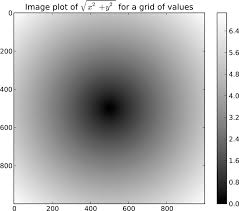
\includegraphics[scale=0.4]{figures/1174051/7/7.png}
\caption{Train Inputs 2}
\end{figure}

\end{itemize}

\subsubsection{Soal No. 8}
 Maksud dari  d train outputs = np utils.to categorical(d[’CLASS’].iloc[train idx]) dan d test outputs = np utils.to categorical(d[’CLASS’].iloc[test idx])

Fungsi pada kode program tersebut ditujukan untuk melakukan one-hot encoding supaya bisa masuk dan digunakan pada neural network. One-hot encoding diambil dari class yang berarti hanya terdapat 2 neuron, yaitu satu nol(1,0) atau nol satu(0,1) karena pilihannya hanya ada dua.

\begin{itemize}
\item Ilustrasi Gambar:

\begin{figure}[H]
\centering
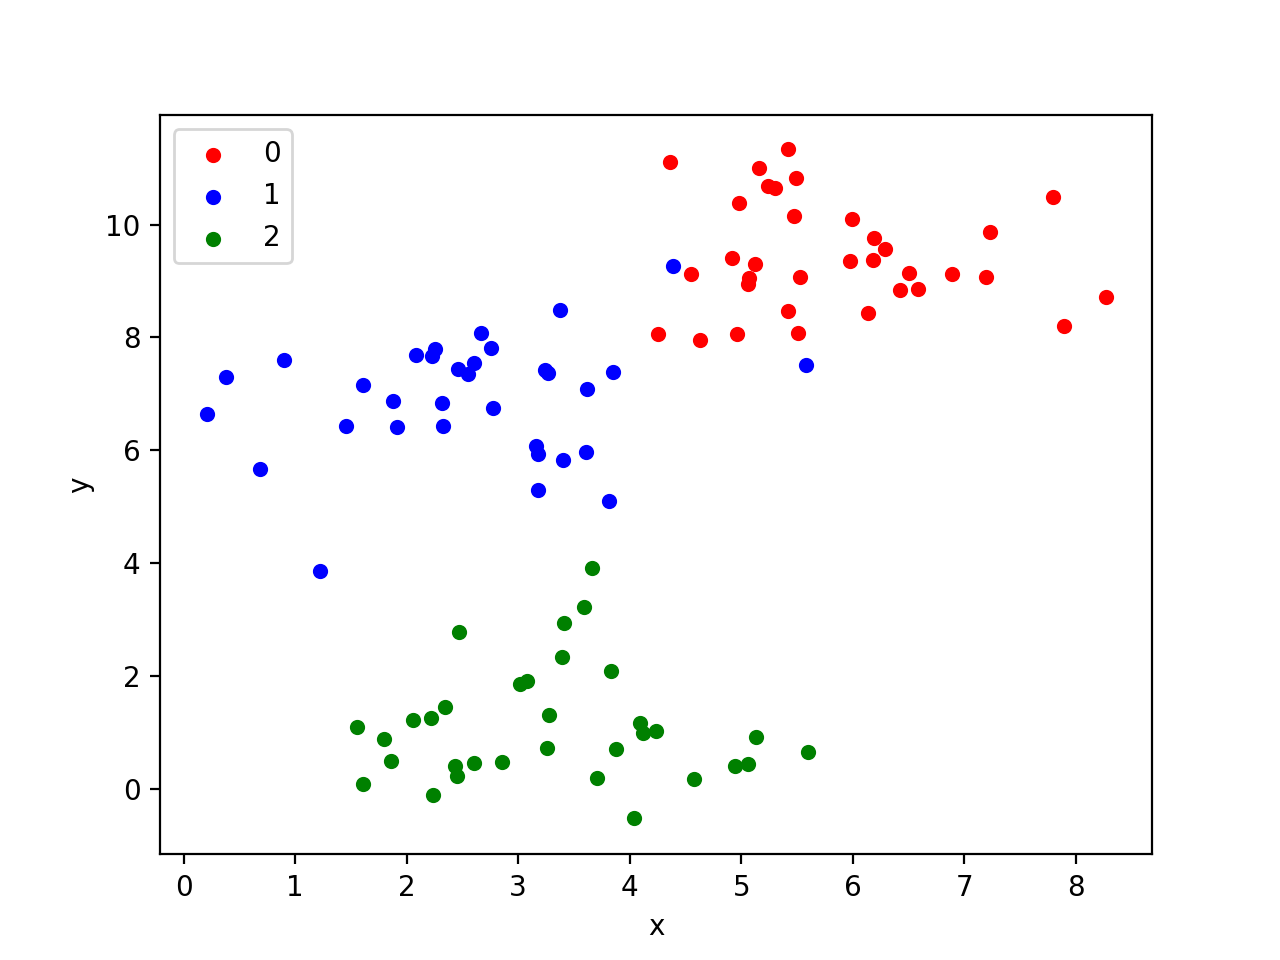
\includegraphics[scale=0.4]{figures/1174051/7/8.png}
\caption{Compile model}
\end{figure}

\end{itemize}

\subsubsection{Soal No. 9}
Maksud dari listing 7.2.

\hfill \break

Fungsi kode program tersebut untuk melakukan pemodelan dengan sequential, membandingkan setiap satu larik elemen dengan cara satu persatu secara beruntun.Terdapat 512 neuron inputan dengan input shape 2000 vektor yang sudah dinormalisasi. Lalu model dilakukan aktivasi dengan fungsi 'relu'. Kemudian pemotongan bobot supaya tidak overfitting sebesar 50 persen dari neuron inputan 512. Lalu pada layer output terdapat 2 neuron outputan yaitu nol (1,0) atau nol satu (0,1). Kemudian outputan tersebut diaktivasi menggunakan fungsi softmax.

\subsubsection{Soal No. 10}
Maksud dari listing 7.3.

\hfill \break

Fungsi kode program tersebut untuk model yang telah dibuat selanjutnya dicompile dengan menggunakan algoritma optimisasi, fungsi loss, dan fungsi metrik.

\subsubsection{Soal No. 11}
Deep Learning

\hfill \break

Deep learning, yang bisa diartikan sebagai rangkaian metode untuk melatih jaringan saraf buatan multi-lapisan. Ternyata, metode ini efektif dalam mengidentifikasi pola dari data. Manakala media membicarakan jaringan saraf, kemungkinan yang dimaksud adalah deep learning.

\subsubsection{Soal No. 12}
Deep Neural Network, dan apa bedanya dengan Deep Learning

\hfill \break

Algoritma DNN (Deep Neural Networks) adalah salah satu algoritma berbasis jaringan saraf yang dapat digunakan untuk pengambilan keputusan. Contoh yang dibahas kali ini adalah mengenai penentuan penerimaan pengajuan kredit sepeda motor baru berdasarkan kelompok data yang sudah ada. 

Pebedaannya dengan Deep Learning adalah terletak pada kedalaman model, deep learning adalah frasa yang digunakan untuk jaringan saraf yang kompleks.

\subsubsection{Soal No. 13}
Jelaskan dengan ilustrasi gambar buatan sendiri, bagaimana perhitungan algoritma konvolusi dengan ukuran stride (NPM mod3+1)x(NPM mod3+1) yang terdapat max pooling.(nilai 30)

Karena NPM saya 1174051 dan hasil dari (NPM mod 3)+1 = 2, maka saya menggunaan matrik kernel berukuran 2x2. Misalkan f(x,y) yang digunakan berukuran 3x3 dan kernel atau mask berukuran 2x2 adalah sebagai berikut:

Gambar Matriks:

\begin{figure}[H]
\centering
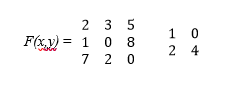
\includegraphics[scale=0.8]{figures/1174051/7/9.png}
\caption{Perhitungan algoritma konvolusi}
\end{figure}

Penyelesaian dari operasi konvolusi antara f(x,y) dengan kernel g(x,y)  adalah f(x,y) *  g(x,y) 

\begin{itemize}
\item  Tempatkan matrik kernel di sebelah kiri atas, lalu hitung nilai piksel pada posisi (0,0) dari kernel tersebut. Konvolusi dihitung dengan cara berikut :

(2x1) + (3x0) + (1x2) + (0x4)

Sehingga didapat hasil konvolusi = 4

\item Tempatkan matrik kernel di sebelah kanan atas, lalu hitung nilai piksel pada posisi (0,0) dari kernel tersebut. Konvolusi dihitung dengan cara berikut :

(3x1) + (5x0) + (0x2) + (8x4)

Sehingga didapat hasil konvolusi = 35

\item Tempatkan matrik kernel di sebelah kiri bawah, lalu hitung nilai piksel pada posisi (0,0) dari kernel tersebut. Konvolusi dihitung dengan cara berikut :

(1x1) + (0x0) + (7x2) + (2x4)

Sehingga didapat hasil konvolusi = 23

\item Tempatkan matrik kernel di sebelah kanan bawah, lalu hitung nilai piksel pada posisi (0,0) dari kernel tersebut. Konvolusi dihitung dengan cara berikut :

(0x1) + (8x0) + (2x2) + (0x4)

Sehingga didapat hasil konvolusi = 4

Hasil:

\begin{figure}[H]
\centering
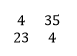
\includegraphics[scale=0.8]{figures/1174051/7/10.png}
\caption{Hasil}
\end{figure}

\end{itemize}

\subsection{Praktek}
\subsubsection{Soal No. 1}
Jelaskan arti dari setiap baris kode program pada blok \# In[1] dan hasil luarannya.

\begin{itemize}
\item Code:
\lstinputlisting{src/1174051/7/1.py}

\item Penjelasan:

Baris Code 1: Memasukkan atau mengimport file csv

Baris Code 2: Memasukkan module image sebagai pil\_image dari library PIL

Baris Code 3: Memasukkan atau mengimport fungsi keras.processing.image 

\item Hasil output:

\begin{figure}[H]
\centering
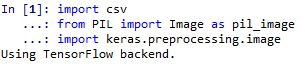
\includegraphics[scale=0.7]{figures/1174051/7/11.jpg}
\caption{1}
\end{figure}

\end{itemize}

\subsubsection{Soal No. 2}
Jelaskan arti dari setiap baris kode program pada blok \# In[2] dan hasil luarannya.

\begin{itemize}
\item Code:
\lstinputlisting{src/1174051/7/2.py}

\item Penjelasan:

Baris Code 1: Membuat variabel imgs tanpa parameter

Baris Code 2: Membuat variabel classes tanpa parameter

Baris Code 3: Membuka file HASYv2/hasy-data-labels.csv

Baris Code 4: Membuat variabel csvreader untuk pembacaan dari file csv yang dimasukkan

Baris Code 5: Membuat variabel i dengan parameter 0

Baris Code 6: Mengeksekusi baris dari pembacaan csv 

Baris Code 7: Mengaplikasikan perintah "if" dengan ketentuan variabel i lebih besar dari angka 0, maka akan dilanjutkan ke perintah berikutnya

Baris Code 8: Membuat variabel img yang mengubah image menjadi bentuk array dari file HASYv2 yang dibuka dengan row berparameter 0.

Baris Code 9: Membuat variabel img atau dengan nilai 255.0

Baris Code 10: Mendefinisikan fungsi imgs.append dimana merupakan proses melampirkan atau menggabungkan data dengan file lain atau set data yang ditentukan dengan 3 parameter yaitu row[0], row[2] dan variabel img.

Baris Code 11: Mendefinisikan fungsi append kembali dari variabel classes dengan parameternya row[2].

Baris Code 12: Mendefinisikan fungsi dimana i variabel i akan ditambah nilainya sehingga akan bernilai 1.

\item Hasil output:

\begin{figure}[H]
\centering
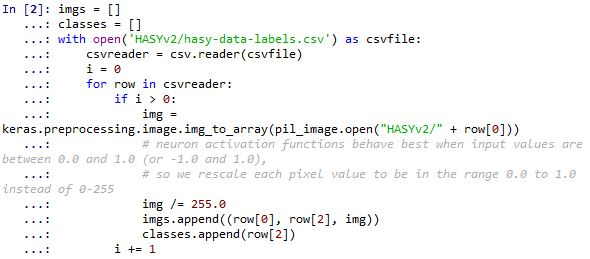
\includegraphics[scale=0.7]{figures/1174051/7/12.jpg}
\caption{2}
\end{figure}

\end{itemize}

\subsubsection{Soal No. 3}
Jelaskan arti dari setiap baris kode program pada blok \# In[3] dan hasil luarannya.

\begin{itemize}
\item Code:
\lstinputlisting{src/1174051/7/3.py}

\item Penjelasan:

Baris Code 1: Memasukkan module random

Baris Code 2: Melakukan pengocokan atau pengacakan pada module random dengan parameter variabelnya imgs

Baris Code 3: Membagi dan memecah index dalam bentuk integer dengan mengkalikan nilai 0,8 dan fungsi len yang akan mengembalikan jumlah item dalam datanya dari variabel imgs

Baris Code 4: Membuat variabel train yang mengeksekusi imgs dengan pemecahan index awal pada data

Baris Code 5: Membuat variabel test yang mengeksekusi imgs dengan pemecahan index akhir pada data

\item Hasil output:

\begin{figure}[H]
\centering
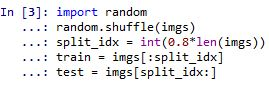
\includegraphics[scale=0.7]{figures/1174051/7/13.jpg}
\caption{3}
\end{figure}

\end{itemize}

\subsubsection{Soal No. 4}
Jelaskan arti dari setiap baris kode program pada blok \# In[4] dan hasil luarannya.

\begin{itemize}
\item Code:
\lstinputlisting{src/1174051/7/4.py}

\item Penjelasan:

Baris Code 1: Mengimport library numpy sebagai np

Baris Code 2: Membuat variabel train\_input untuk input menjadi sebuah array dari np menggunakan fungsi list untuk mengkoleksikan data yang dipilih dan diubah. Didalamnya diterapkan fungsi map untuk mengembalikan iterator dari datanya dengan memfungsikan lamda pada row dengan parameter [2] untuk membuat objek fungsi menjadi lebih kecil dan mudah dieksekusi dari variabel train.

Baris Code 3: Membuat variabel test\_input dengan fungsi seperti train\_input yang membedakan hanya datanya atau inputan yang diproses berasal dari variabel test

Baris Code 4: Membuat variabel train\_output untuk mengubah keluaran menjadi sebuah array dari np dengan menggunakan fungsi list untuk mengkoleksi data yang dipilih dan diubah. Didalamnya diterapkan fungsi map untuk mengembalikan iterator dari datanya dengan memfungsikan lamda pada row dengan parameter[1] untuk membuat objek fungsi menjadi lebih kecil dan mudah dieksekusi dari variabel train.

Baris Code 5: Membuat variabel test\_output dengan fungsi yang sama seperti train\_output yang membedakan hanya datanya atau inputan yang diproses berasal dari variabel test

\item Hasil output:

\begin{figure}[H]
\centering
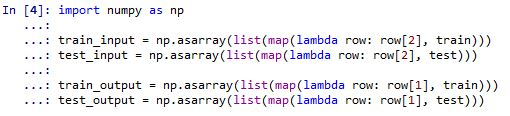
\includegraphics[scale=0.7]{figures/1174051/7/14.jpg}
\caption{4}
\end{figure}

\end{itemize}

\subsubsection{Soal No. 5}
Jelaskan arti dari setiap baris kode program pada blok \# In[5] dan hasil luarannya.

\begin{itemize}
\item Code:
\lstinputlisting{src/1174051/7/5.py}

\item Penjelasan:

Baris Code 1: Memasukkan modul atau fungsi LabelEncoder dari sklearn.processing untuk dapat digunakan menormalkan label dimana label encoder didefinisikan dengan nilai antara 0 dan n\_classes-1.

Baris Code 2: Memasukkan modul atau fungsi OneHotEncoder dari sklearn.processing untuk mendefinisikan fitur input dimana mengambil nilai dalam kisaran [0, maks (nilai)).

\item Hasil output:

\begin{figure}[H]
\centering
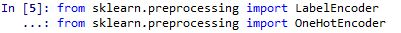
\includegraphics[scale=0.7]{figures/1174051/7/15.jpg}
\caption{5}
\end{figure}

\end{itemize}

\subsubsection{Soal No. 6}
Jelaskan arti dari setiap baris kode program pada blok \# In[6] dan hasil luarannya.

\begin{itemize}
\item Code:
\lstinputlisting{src/1174051/7/6.py}

\item Penjelasan:

Baris Code 1: Membuat variabel label\_encoder dengan modul atau fungsi dari LabelEncoder tanpa parameter

Baris Code 2: Membuat variabel integer\_encoded dengan fungsi label\_encoder.fit\_transform dari variabel classes yang akan mengembalikan beberapa data yang diubah kembali dari variabel label\_encoder.

\item Hasil output:

\begin{figure}[H]
\centering
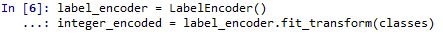
\includegraphics[scale=0.7]{figures/1174051/7/16.jpg}
\caption{6}
\end{figure}

\end{itemize}

\subsubsection{Soal No. 7}
Jelaskan arti dari setiap baris kode program pada blok \# In[7] dan hasil luarannya.

\begin{itemize}
\item Code:
\lstinputlisting{src/1174051/7/7.py}

\item Penjelasan:

Baris 1: Membuat variabel onehot\_encoder yang memanggil fungsi OneHotEncoder tanpa mengembalikan matriks karena sparse=false.

Baris 2: Membuat variabel integer\_encoded memanggil variabel integer\_encoded pada kode program 6 untuk dieksekusi memberikan bentuk baru ke array tanpa mengubah datanya dari mengembalikan panjang nilai dari integer\_encoded.

Baris 3: Onehotencoding melakukan fitting pada integer\_encoded.

\item Hasil output:

\begin{figure}[H]
\centering
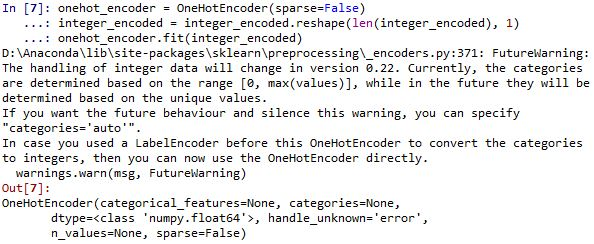
\includegraphics[scale=0.7]{figures/1174051/7/17.jpg}
\caption{7}
\end{figure}

\end{itemize}

\subsubsection{Soal No. 8}
Jelaskan arti dari setiap baris kode program pada blok \# In[8] dan hasil luarannya.

\begin{itemize}
\item Code:
\lstinputlisting{src/1174051/7/8.py}

\item Penjelasan:

Baris 1: Membuat variabel train\_output\_int yang mengeksekusi label\_encoder dengan mengubah nilai dari parameter variabel train\_output.

Baris 2: Membuat variabel train\_output yang mengeksekusi variabel onehot\_encoder dari kode program 7 dengan mengubah nilai dari variabel parameter train\_output\_int yang datanya sudah diubah kedalam bentuk array dan panjang nilai dari train\_output\_int telah dikembalikan.

Baris 3: Membuat variabel test\_output\_int yang mengeksekusi label\_encoder dengan mengubah nilai dari parameter variabel test\_output.

Baris 4: Membuat variabel test\_output yang mengeksekusi variabel onehot\_encoder dari kode program 7 dengan mengubah nilai dari variabel parameter test\_output\_int yang datanya sudah diubah kedalam bentuk array dan panjang nilai dari test\_output\_int telah dikembalikan.

Baris 5: Membuat variabel num\_classes untuk mengetahui jumlah class dari lebel\_encoder

Baris 6: Perintah print digunakan untuk memunculkan hasil dari variabel num\_classes

\begin{figure}[H]
\centering
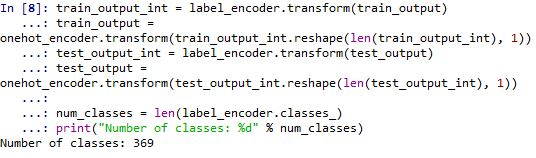
\includegraphics[scale=0.7]{figures/1174051/7/18.jpg}
\caption{8}
\end{figure}

\item Hasil output:

\end{itemize}

\subsubsection{Soal No. 9}
Jelaskan arti dari setiap baris kode program pada blok \# In[9] dan hasil luarannya.

\begin{itemize}
\item Code:
\lstinputlisting{src/1174051/7/9.py}

\item Penjelasan:

Baris 1: Melakukan importing fungsi model sequential dari library keras.

Baris 2: Melakukan importing fungsi layer dense, dropout, dan flatten dari library keras.

Baris 3: Melakukan importing fungsi layer Conv2D dan MaxPooling2D dari library keras.

\item Hasil output:

\begin{figure}[H]
\centering
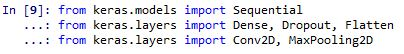
\includegraphics[scale=0.7]{figures/1174051/7/19.jpg}
\caption{9}
\end{figure}

\end{itemize}

\subsubsection{Soal No. 10}
Jelaskan arti dari setiap baris kode program pada blok \# In[10] dan hasil luarannya.

\begin{itemize}
\item Code:
\lstinputlisting{src/1174051/7/10.py}

\item Penjelasan:

Baris 1: Melakukan pemodelan Sequential.

Baris 2: Menambahkan Konvolusi 2D dengan 32 filter konvolusi masing-masing berukuran 3x3 dengan algoritam activation relu dengan data dari train input mulai dari baris nol.

Baris 3: Menambahkan Max Pooling dengan matriks 2x2.

Baris 4: Penambahan Konvolusi 2D dengan 32 filter, konvolusi masing-masing berukuran 3x3 dengan algoritam activation relu.

Baris 5 Menambahkan Max Pooling dengan matriks 2x2.

Baris 6: Mendefinisikan inputan dengan 1024 neuron dan menggunakan algoritma tanh untuk activationnya.

Baris 7: Dropout terdiri dari pengaturan secara acak tingkat pecahan unit input ke 0 pada setiap pembaruan selama waktu pelatihan, yang membantu mencegah overfitting sebesar 50\% .

Baris 8: Untuk output layer menggunakan data dari variabel num classes dengan fugsi activationnya softmax.

Baris 9: Konfigurasi proses pembelajaran, melalui metode compile, sebelum melatih suatu model.

Baris 10: Menampilkan model yang telah dibuat.

\item Hasil output:

\begin{figure}[H]
\centering
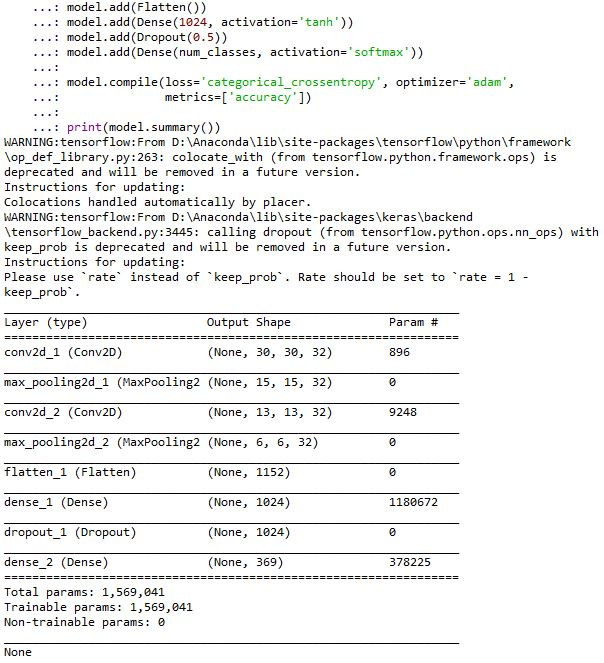
\includegraphics[scale=0.7]{figures/1174051/7/20.jpg}
\caption{10}
\end{figure}

\end{itemize}

\subsubsection{Soal No. 11}
Jelaskan arti dari setiap baris kode program pada blok \# In[11] dan hasil luarannya.

\begin{itemize}
\item Code:
\lstinputlisting{src/1174051/7/11.py}

\item Penjelasan:

Baris Code 1:  Melakukan import library keras.callbacks yang digunakan pada penulisan log untuk TensorBoard, untuk memvisualisasikan grafik dinamis dari pelatihan dan metrik pengujian.

Baris Code 2: Membuat variabel tenserboard untuk mendefinisikan fungsi TensorBoard pada keras.callbacks yang digunakan sebagai alat visualisasi yang disediakan dengan TensorFlow. Dan untuk fungsi log\_dir memanggil data yaitu './logs/mnist-style'

\item Hasil output:

\begin{figure}[H]
\centering
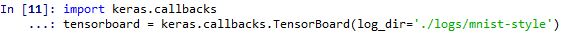
\includegraphics[scale=0.7]{figures/1174051/7/21.jpg}
\caption{11}
\end{figure}

\end{itemize}

\subsubsection{Soal No. 12}
Jelaskan arti dari setiap baris kode program pada blok \# In[12] dan hasil luarannya.

\begin{itemize}
\item Code:
\lstinputlisting{src/1174051/7/12.py}

\item Penjelasan:

Baris Code 1: Menerapkan fungsi model.fit yang didalamnya memproses train\_input, train\_output

Baris Code 2: Penerapan fungsi yang sama difungsikan batch\_size apabila batch\_sizenya tidak ditemukan maka otomatis akan dijadikan nilai 32

Baris Code 3: Penerapan fungsi yang sama, difungsikan epochs dimana perulangan dari berapa kali nilai yang digunakan untuk data, dan jumlahnya ialah 10

Baris Code 4: Mendefinisikan fungsi verbose untuk digunakan sebagai opsi menghasilkan informasi logging dari data yang ditentukan dengan nilai 2

Baris Code 5: Mendefinisikan fungsi validation\_split untuk memecah nilai dari perhitungan validasinya sebesar 0,2. (Fraksi data pelatihan untuk digunakan sebagai data validasi)

Baris Code 6: Mendefinisikan fungsi callsbacks dengan parameternya yang mengeksekusi tensorboard dimana digunakan untuk visualisasikan parameter training, metrik, hiperparameter pada nilai/data yang diproses

Baris Code 7: Mendefinisikan variabel score dengan fungsi evaluate dari model dengan parameter test\_input, tst\_output dan verbose=2 untuk memprediksi output dan input yang diberikan dan kemudian menghitung fungsi metrik yang ditentukan dalam modelnya

Baris Code 8: Mencetak score optimasi dari test dengan ketentuan nilai parameter 0

Baris Code 9: Mencetak score akurasi dari test dengan ketentuan nilai parameter 1

\item Hasil output:

\begin{figure}[H]
\centering
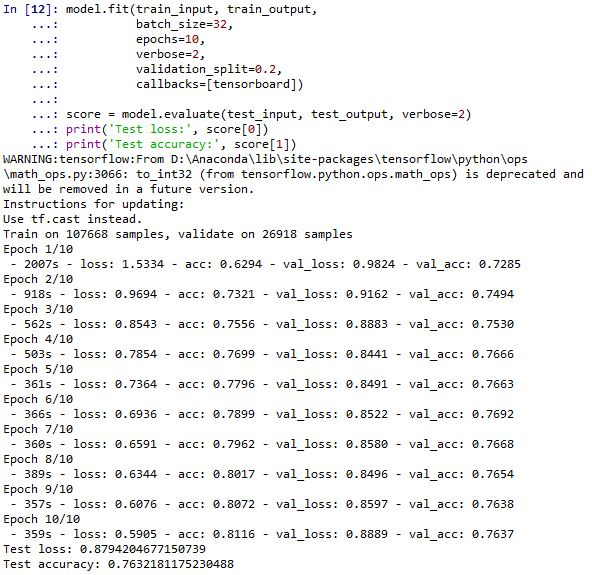
\includegraphics[scale=0.7]{figures/1174051/7/22.jpg}
\caption{12}
\end{figure}

\end{itemize}

\subsubsection{Soal No. 13}
Jelaskan arti dari setiap baris kode program pada blok \# In[13] dan hasil luarannya.

\begin{itemize}
\item Code:
\lstinputlisting{src/1174051/7/13.py}

\item Penjelasan:

Baris 1: Import atau memasukkan modul time

Baris 2: Variabel result berisikan array kosong

Baris 3: Menggunakan convolution 2D yang berarti memiliki 1 atau 2 layer

Baris 4: Mendefinisikan dense size dengan ukuran 128, 256, 512, 1024, 2048

Baris 5: Mendefinsikan drop out dengan 0, 25\%, 50\%, dan 75\%

Baris 6: Melakukan pemodelan Sequential

Baris 7: Jika ini adalah layer pertama, akan memasukkan bentuk input.

Baris 8: Kalau tidak kita hanya akan menambahkan layer.

Baris 9: Kemudian, setelah menambahkan layer konvolusi, lakukan hal yang sama dengan max pooling.

Baris 10: Lalu, ratakan atau flatten dan menambahkan dense size ukuran apa pun yang berasal dari dense size. Dimana akan selalu menggunakan algoritma tanh

Baris 11: Jika dropout digunakan, akan menambahkan layer dropout. Dropout ini berarti misalnya 50\%, bahwa setiap kali memperbarui bobot setelah setiap batch, ada peluang 50\% untuk setiap bobot yang tidak akan diperbarui

Baris 12: Menempatkan di antara dua lapisan padat untuk dihidupkan dari melindunginya dari overfitting. Lapisan terakhir akan selalu menjadi jumlah kelas karena itu harus, dan menggunakan softmax. Itu dikompilasi dengan cara yang sama.

Baris 13: Atur direktori log yang berbeda untuk TensorBoard sehingga dapat membedakan konfigurasi yang berbeda.

Baris 14: Variabel start akan memanggil modul time

Baris 15: Melakukan fit atau compile

Baris 16: Melakukan scoring dengan evaluate yang akan menampilkan data loss dan accuracy dari model

Baris 17: 'End' merupakan variabel untuk melihat waktu akhir pada saat pemodelan berhasil dilakukan.

Baris 18: Menampilkan hasil dari skrip diatas

\item Hasil output:

\begin{figure}[H]
\centering
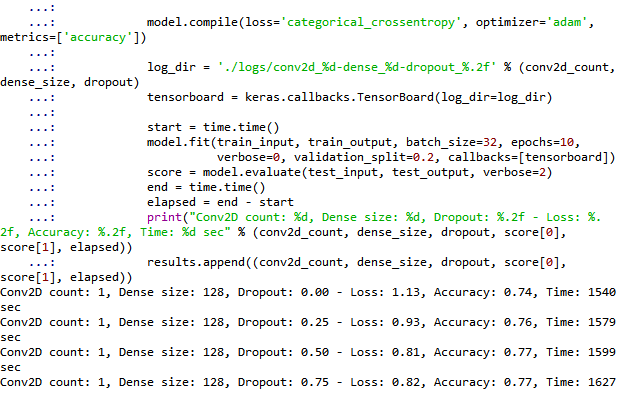
\includegraphics[scale=0.7]{figures/1174051/7/23.png}
\caption{13}
\end{figure}

\end{itemize}

\subsubsection{Soal No. 14}
Jelaskan arti dari setiap baris kode program pada blok \# In[14] dan hasil luarannya.

\begin{itemize}
\item Code:
\lstinputlisting{src/1174051/7/14.py}

\item Penjelasan:

Baris 1: Melakukan pemodelan Sequential

Baris 2: Menambahkan Convolutio 2D dengan dmensi 32, dan ukuran matriks 3x3 dengan function aktivasi yang digunakan yaitu relu dan menampilkan input shape

Baris 3: Melakukan Max Pooling 2D dengan ukuran matriks 2x2

Baris 4: Melakukan Convolusi lagi dengan kriteria yang sama tanpa menambahkan input, ini dilakukan untuk mendapatkan data yang terbaik

Baris 5: Flatten digunakan untuk meratakan inputan atau masukkan data

Baris 6: Menambahkan dense input sebanyak 128 neuron dengan menggunakan function aktivasi tanh.

Baris 7: Dropout sebanyak 50\% untuk menghindari overfitting

Baris 8: Menambahkan dense pada model untuk output dimana layerini akan menjadi jumlah dari class yang ada.

Baris 9: Mengcompile model yang didefinisikan diatas

Baris 10: Menampilkan ringkasan dari pemodelan yang dilakukan

\item Hasil output:

\begin{figure}[H]
\centering
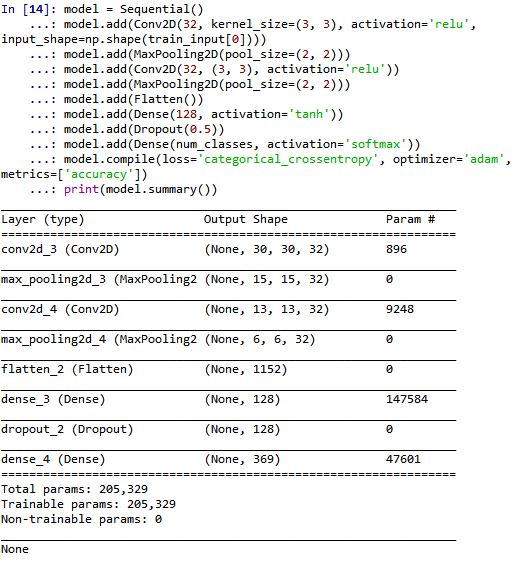
\includegraphics[scale=0.7]{figures/1174051/7/24.jpg}
\caption{14}
\end{figure}

\end{itemize}

\subsubsection{Soal No. 15}
Jelaskan arti dari setiap baris kode program pada blok \# In[15] dan hasil luarannya.

\begin{itemize}
\item Code:
\lstinputlisting{src/1174051/7/15.py}

\item Penjelasan:

Baris 1: Melakukan fit dengan join data train dan test agar dapat dilakukan pelatihan untuk jaringan pada smeua data yang dimiliki.

\item Hasil output:

\begin{figure}[H]
\centering
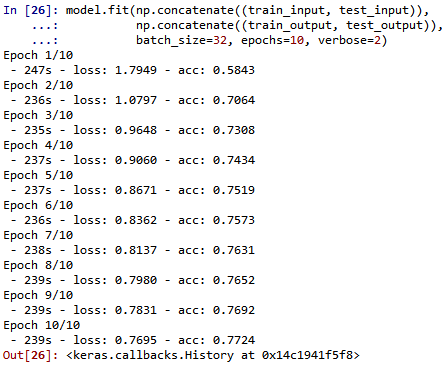
\includegraphics[scale=0.7]{figures/1174051/7/25.png}
\caption{15}
\end{figure}

\end{itemize}

\subsubsection{Soal No. 16}
Jelaskan arti dari setiap baris kode program pada blok \# In[16] dan hasil luarannya.

\begin{itemize}
\item Code:
\lstinputlisting{src/1174051/7/16.py}

\item Penjelasan:

Baris 1: Menyimpan model yang telah di latih dengan nama mathsymbols.model

\item Hasil output:

\begin{figure}[H]
\centering
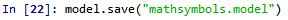
\includegraphics[scale=0.7]{figures/1174051/7/26.jpg}
\caption{16}
\end{figure}

\end{itemize}

\subsubsection{Soal No. 17}
Jelaskan arti dari setiap baris kode program pada blok \# In[17] dan hasil luarannya.

\begin{itemize}
\item Code:
\lstinputlisting{src/1174051/7/17.py}

\item Penjelasan:

Baris 1: Menyimpan label enkoder (untuk membalikkan one-hot encoder) dengan nama classes.npy

\item Hasil output:

\begin{figure}[H]
\centering
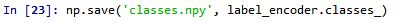
\includegraphics[scale=0.7]{figures/1174051/7/27.jpg}
\caption{17}
\end{figure}

\end{itemize}

\subsubsection{Soal No. 18}
Jelaskan arti dari setiap baris kode program pada blok \# In[18] dan hasil luarannya.

\begin{itemize}
\item Code:
\lstinputlisting{src/1174051/7/18.py}

\item Penjelasan:

Baris 1: Memasukkan atau mengimport models dari librari Keras

Baris 2: Variabel model2 akan memanggil model yang telah disave sebelumnya

Baris 3: Menampilkan ringkasan dari hasil pemodelan

\item Hasil output:

\begin{figure}[H]
\centering
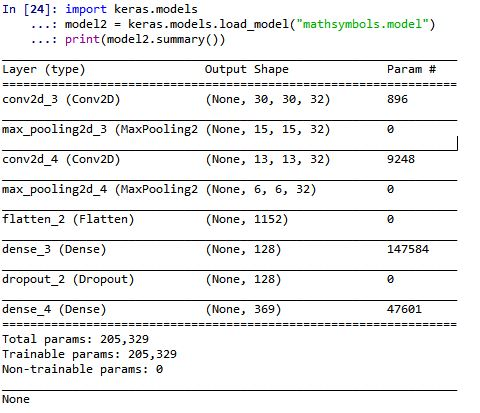
\includegraphics[scale=0.7]{figures/1174051/7/28.jpg}
\caption{18}
\end{figure}

\end{itemize}

\subsubsection{Soal No. 19}
Jelaskan arti dari setiap baris kode program pada blok \# In[19] dan hasil luarannya.

\begin{itemize}
\item Code:
\lstinputlisting{src/1174051/7/19.py}

\item Penjelasan:

Baris 1: Memanggil fungsi LabelEncoder

Baris 2: Variabel label encoder akan memanggil class yang disimpan sebelumnya.

Baris 3: Function Predict akan mengubah gambar kedalam bentuk array

Baris 4: Variabel prediction akan melakukan prediksi untuk model2 dengan reshape variabel newimg dengan bentukarray 4D.

Baris 5: Variabel inverted akan mencari nilai tertinggi output dari hasil prediksi tadi

\item Hasil output:

\begin{figure}[H]
\centering
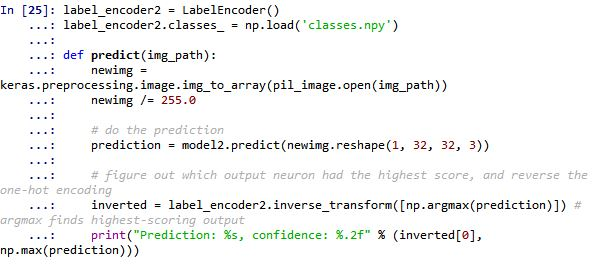
\includegraphics[scale=0.7]{figures/1174051/7/29.jpg}
\caption{19}

\end{figure}

\end{itemize}

\subsubsection{Soal No. 20}
Jelaskan arti dari setiap baris kode program pada blok \# In[20] dan hasil luarannya.

\begin{itemize}
\item Code:
\lstinputlisting{src/1174051/7/20.py}

\item Penjelasan:

Baris 1: Melakukan prediksi dari pelatihan dari gambar v2-00010.png

Baris 2: Melakukan prediksi dari pelatihan dari gambar v2-00500.png

Baris 3: Melakukan prediksi dari pelatihan dari gambar v2-00700.png

\item Hasil output:

\begin{figure}[H]
\centering
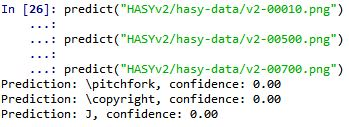
\includegraphics[scale=0.7]{figures/1174051/7/30.jpg}
\caption{20}
\end{figure}

\end{itemize}


\subsection{Penanganan Error}

\subsubsection{Penanganan Error}

\begin{itemize}
\item Screenshoot:
\begin{figure}[H]
\centering
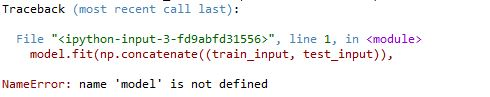
\includegraphics[scale=0.7]{figures/1174051/7/Error.jpeg}
\caption{Error}
\end{figure}

\item Code Error:

NameError: name 'model' is not defined

\item Penanganan Error:

Berdasarkan error maka penyelesaiannya ialah melakukan pendefinisian variabel model sehingga code dapat dijalankan. Lakukan running pada code yang berada diatasnya dimana mendefinisikan variabel model.

\end{itemize}
